\section{The basics of the nervous system.}

The nervous system is the most complex chemical machine known and to be known. Every attempt to study it is condemned to constant theoretical gaps and wide borders, most of them in perpetual darkness. This condition arises from an organizational complexity and not a fundamental one, as the individual elements that comprise it are mostly well understood. Ignoring neuroscience's limitations as a novel field, the knowledge of perception is limited by metaphysical matters. Even after the reader has accepted his own existance, some dilemmas are put into place: there are cases of patients who have suffered cerebral injuries and show changes in behavior such that they become unrecognisable to their loved ones. Trying to explain such phenomena using high abstraction concepts like \enquote{personality} or \enquote{soul} is interesting as intellectual foreplay, but is also a well of contradictory answers. For that reason, when studying these phenomena we can't but limit ourselves to finding patterns in that which we can observe and write a great \enquote{WE DON'T KNOW} in what surrounds it.  

What comes now isn't going to be simple, but in essence it summarizes into:

\begin{enumerate}
	\item The nervous system is made up of cells called neurons.
	\item A neuron can communicate with others through one-directional signals.
	\item Chains and webs of neurons compose functional circuits that can configure simple behaviors (like moving a leg by reflex) up to very complex ones (like emotional state).
\end{enumerate}

Altering the behavior of groups of neurons in very subtle ways can cause chain reactions noticeable at larger scales. This is what happens after administering a drug, and will be seen in detail proximately.

\subsection{The building blocks of the nervous system.}

Entering his thirties and in search for economic stability, Camilo Golgi started to work in a hospital for chronic patients in Abbiategrasso. In his drawer's kitchen, with no more than a microscope and self payed utensils, he built a laboratory to which he came back after taking care of his patients to investigate about a mystery that chased him: the entity responsible for nervous communication. Golgi had discovered a method with which he managed to dye some nervous system's cells in a black color. This histological discovery played with the posibility of understanding the mind, something inimaginable in the 19th century. Ironically, he became eclipsed by the Spanish scientist Santiago Ramón y Cajal who, using his method, elaborated theories much better than his own.

These cells --- called nerve cells or neurons --- had a branching interconnected structure which formed wide networks. Both scientists disagreed on a simple detail: were neurons independent cells as Cajal thought or did they act as a continuous tissue without internal separation as Golgi thought? This confrontation was closed definitely with the invention of electron microscopy and the discovery of a small gap between neurons: the synaptic space (Figure \ref{synapse}-C$_1$).

\begin{figure}[H]
	\centering

	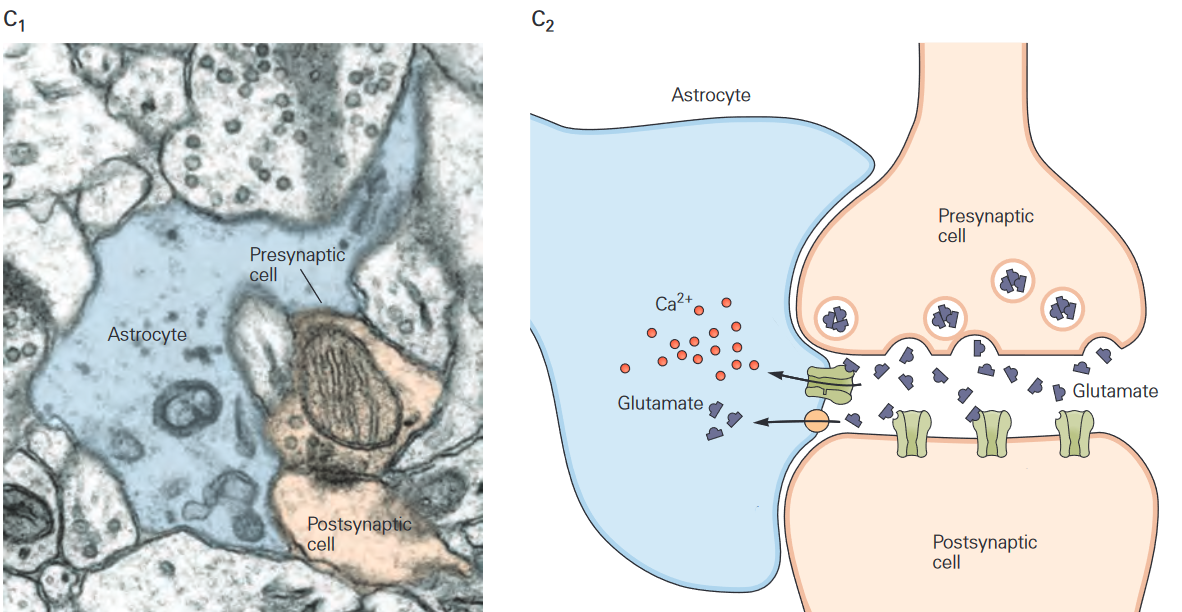
\includegraphics[width=\linewidth]{media/3-synapse.png}
	\caption{(C$_1$) Cells from the nervous system seen under an electron microscope. In orange, neurons separated by the synaptic gap. In blue, an astrocyte that supplies them. (C$_2$) Schematic view. Upon an action potential, calcium channels open. Calcium induces the fusion of synaptic vesicles with the cell membrane (exocitosis), freeing neurotransmitters (glutamate) into the synaptic space. Neurotransmitters join to receptors on the postsynaptic neuron, causing many possible effects. Then they are taken back by the neuron or by the astrocyte.}
	\label{synapse}
\end{figure}

This conflict was however the product of a war that was being fought since Descartes' times. The war between those who thought of the nervous system as a whole and those who thought it was divided into functional, localized parts. Sideproducts of this fight were people like Franz Joseph Gall, who using his theory for the localization of parts, ideated phrenology: a method to determine personality through the measurement of the head's shape which was later used by racism theorists as a scientific justification (Figure \ref{gall}). This idea was opposed to opinions like those from Pierre Fluorens who, testing out Gall's thesis, concluded that all of the brain's parts took care of all mental operations. A reaction not only scientific in nature but cultural, as the reduction of the soul to the internal activity of a network of organs was something unacceptable for the european context.

\begin{figure}[H]
	\centering

	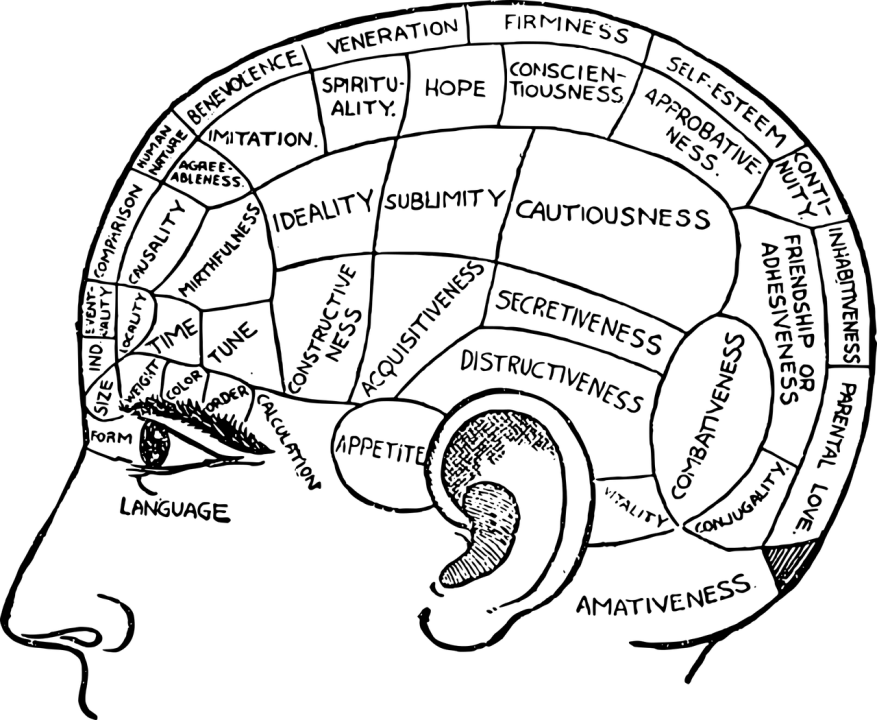
\includegraphics[width=\linewidth]{media/4-gall.png}
	\caption{Functional map of the head according to Franz Joseph Gall. His methods to associate regions and functions were quite poor and his theories were proven wrong, but the idea of using craneum measurements as personality indicators was used as a base for racist theories.}
	\label{gall}
\end{figure}

Current thinking of this is somewhat mixed. While it is recognized that very complex tasks like emotions are performed by many distributed circuits on varied regions, it is also accepted that these can be broken down into much simpler tasks which are generally localizable.

\subsection{Structure and organization.}

The environment provides organisms with a continuous stream of information: electromagnetic radiation, variations in air pressure, vibrations on the ground... There exist organs with receptors capable of reacting to these variations in the environment: the sensory organs. These variations perceived by an organism through these organs are named \textit{stimuli} (note that depending on the level of abstraction, a stimulus can be anything from the ring of a bell to the impact of a single photon). When a sensory organ receives a stimulus, it produces a signal on the nervous system which generally ends up with the activation of another organ which we name \textit{effector}. The action that gets carried out is named \textit{response}, and if the response is complex enough, we call it \textit{behavior}.

Between the stimulus and the response lies the nervous system: a set of cells which conduct electrical signals through different parts of the organism. It is divided in \textit{central nervous system} (CNS), made up of the encephalon and the spinal cord, and \textit{peripheral nervous system} (PNS), made up of all the nerves that branch from the latter. The PNS acts as a highway of information between the CNS and the effector and sensory organs, whereas the CNS takes charge of integrating and processing the contributions of the PNS to offer an adequate response.

For example, upon the presence of a tarantula in one's leg (stimulus), sensory receptors in the skin will send signals communicating the information to the CNS via chains of neurons (nerves) from the PNS. After looking at the tarantula, the CNS, configurated throughout years by past experiences with arachnids, cultural notions on tarantulas or by mere genetic predisposal may activate through the PNS muscles from the leg to shake it and glands to secrete stress and fear hormones. The PNS has then two ways: an \textit{afferent} one (from the sensory organs to the CNS) and an \textit{efferent} one (from the CNS to the effector organs).

Not all responses require the encephalon. Many reflex behaviors are self-contained in the spinal cord's circuitry . However, the encephalon offers a very useful capacity for interpretation in more complex living things.

The cells from the nervous system which send and receive signals are the neurons (Figure \ref{neuron}), but in the nervous system there are also many other cells like glia, which serve as support for neurons (Figure \ref{glia}). From microglia, with immunitary function, to macroglia, which covers neurons with a lipidic layer of mielin, nourishes them by controlling the pass of substances from the bloodstream and controls the concentrations of ions, neurotransmitters and exogenous elements (Figure \ref{synapse}).

\begin{figure}[H]
	\centering
	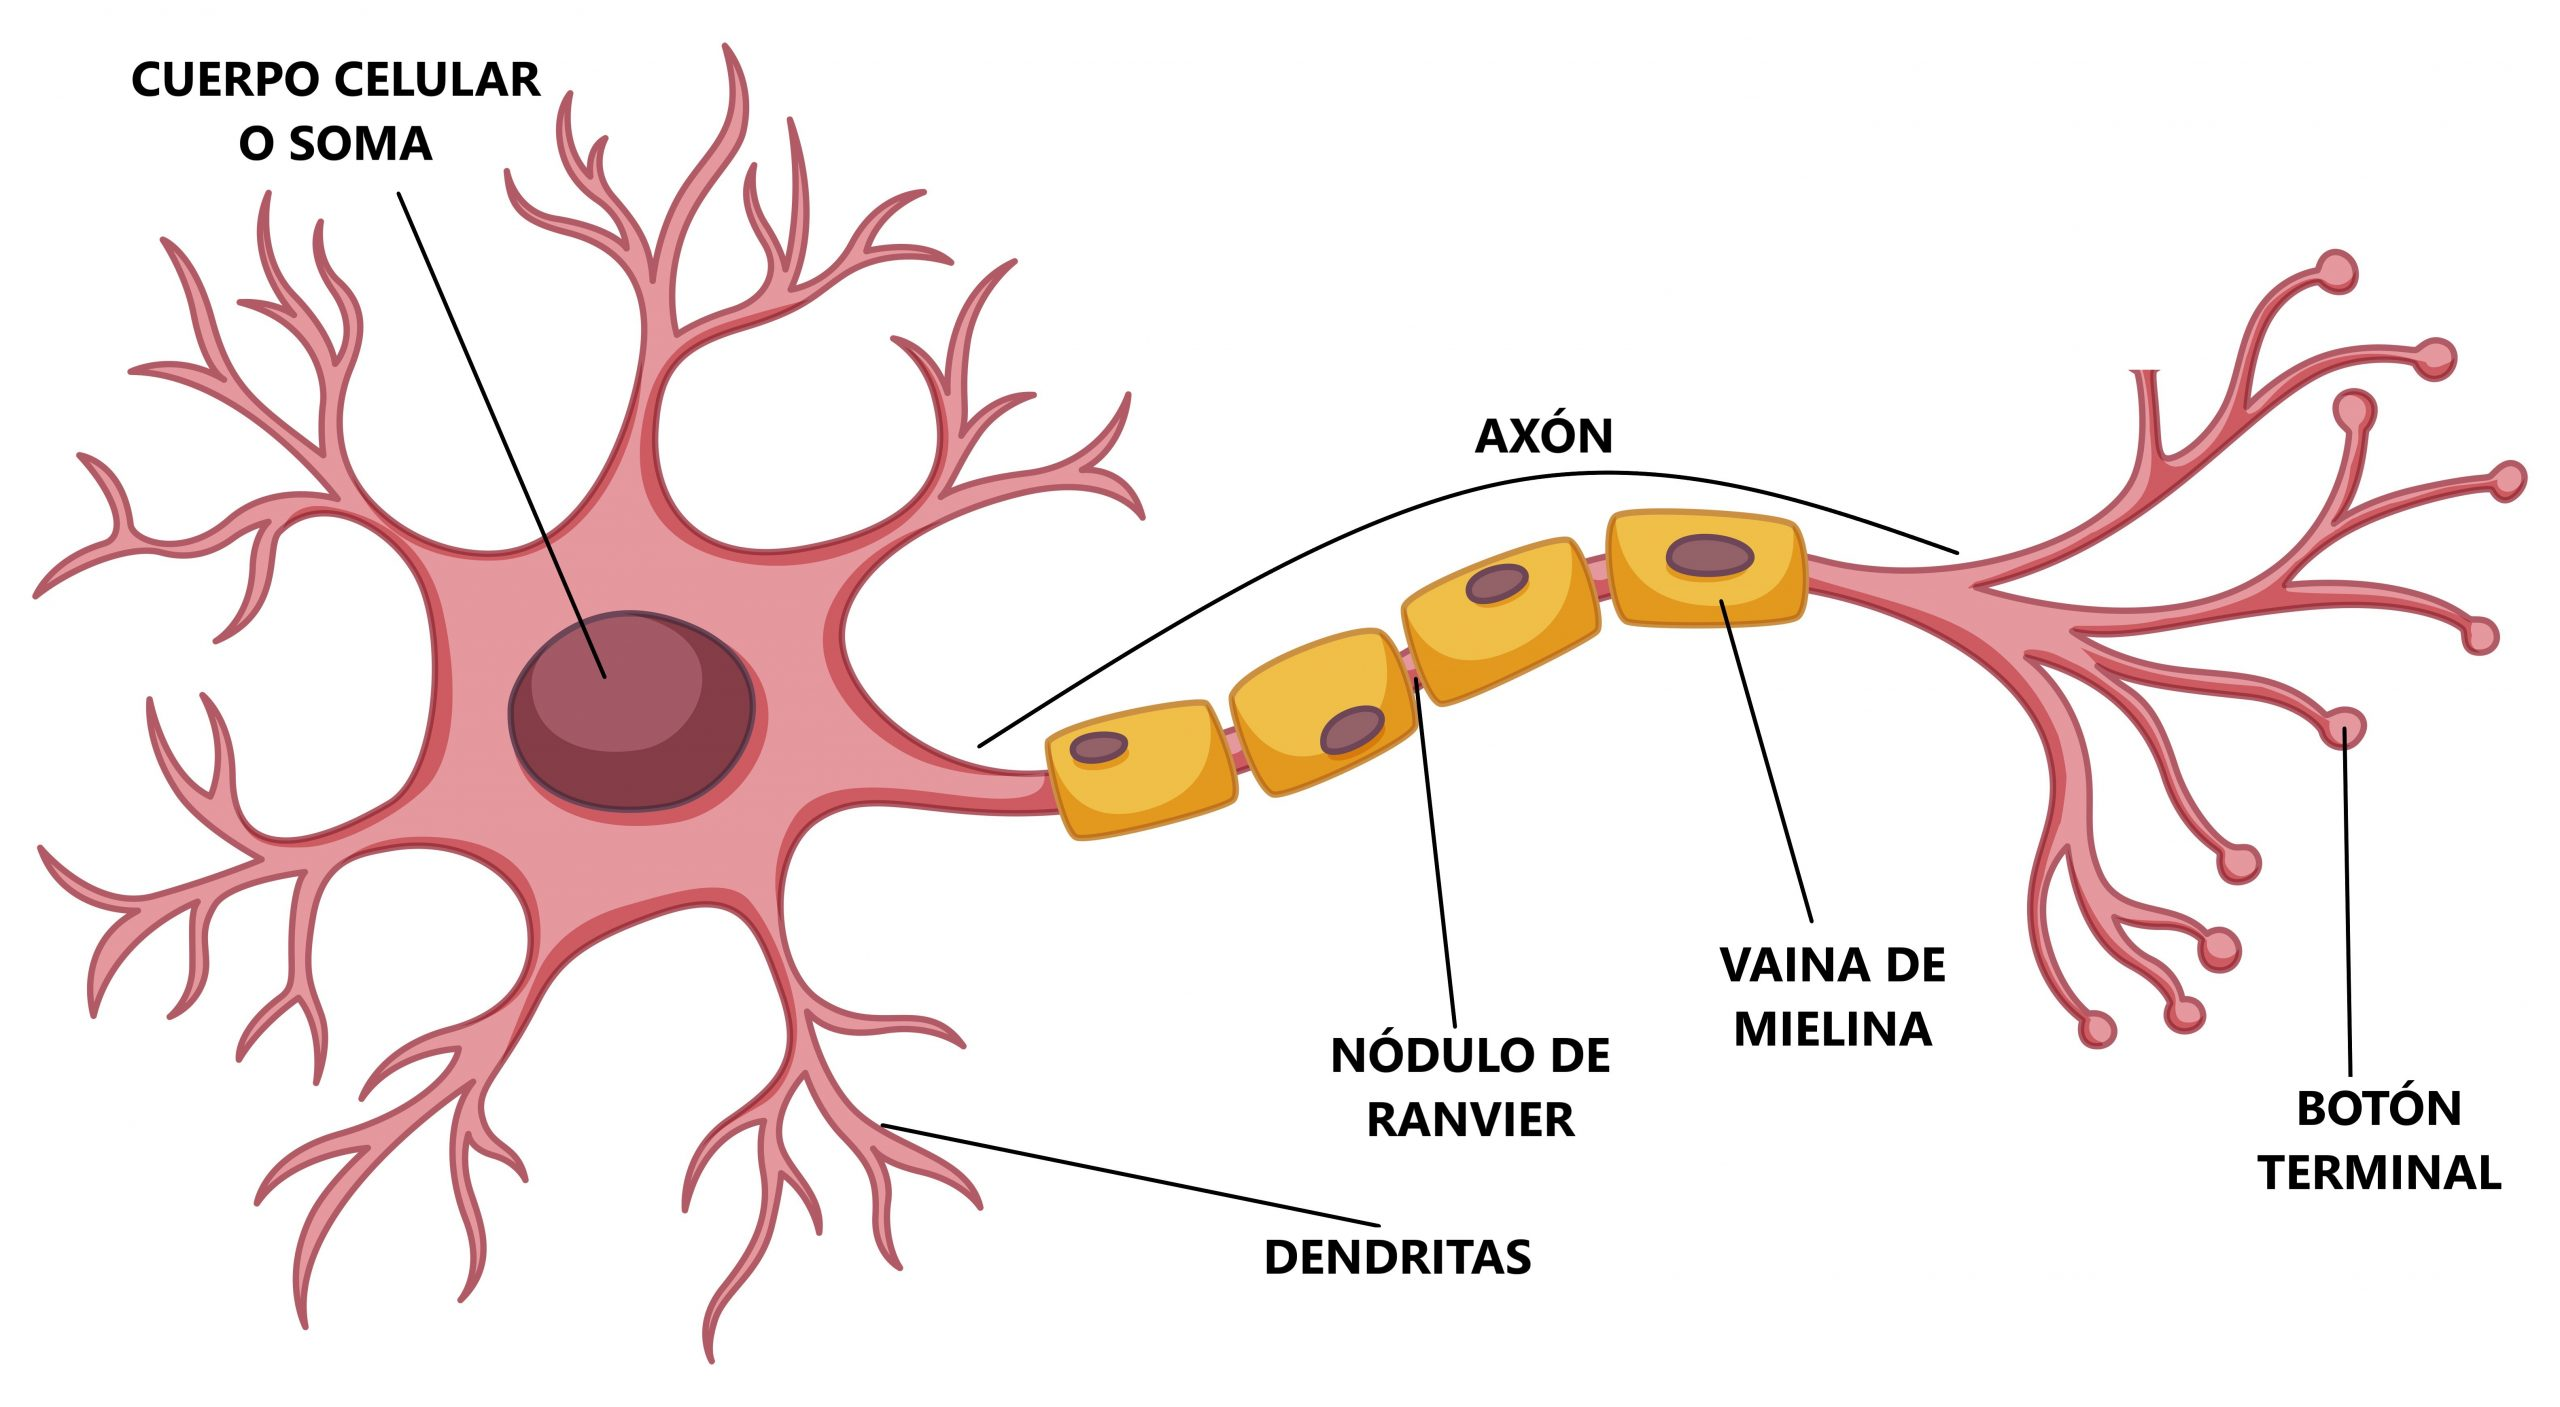
\includegraphics[width=\linewidth]{media/5-neuron.jpg}
	\caption{The neuron.}
	\label{neuron}
\end{figure}

\begin{figure}[H]
	\centering

	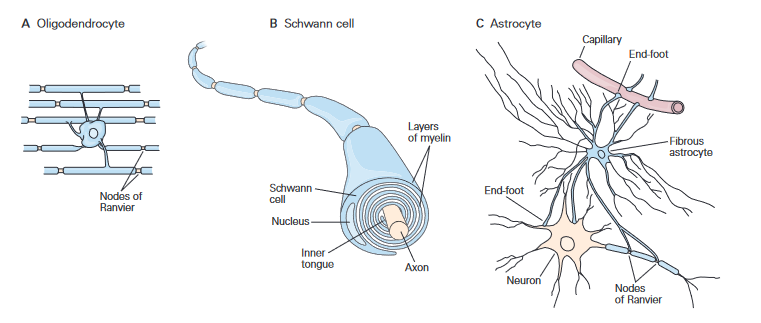
\includegraphics[width=\linewidth]{media/5-glia.png}
	\caption{Macroglial cells.}
	\label{glia}
\end{figure}

\subsection{The neuron.}

Every neuron is composed of three parts: a soma or cell body, where the metabolic processes common to every cell happen; the dendrites, a branched structure through which signals enter; and the axon, also branched and which sends signals to other neurons. The axon carries out an integrating function, as based on the many received signals it \enquote{decides} whether or not to fire a signal to other neurons. The neuron that sends a signal is called \textit{presynaptic neuron}, and the one that receives it is called \textit{postsynaptic neuron}. Obviously these are relative terms, as every neuron is both presynaptic and postsynaptic. How is the very fast communication observed in the nervous system possible? A molecular analysis is required.

At rest state the neuron is polarized, that is, just as a battery, it constantly mantains a difference in electric potential between its interior and its exterior of about 70 milivolts less. We say the interior is at -70 mV with respect to the exterior. Where does this potential come from and why isn't there an instant short circuit which calms it? It all depends on a delicate equilibrium (Figure \ref{action}).

As every cell is, the neuron is also delimited by a phospholipid bilayer, and hence it doesn't allow the transit of charged substances like ions. Because ions can't pass through, the flow of electricity is impossible, and so the aforementioned short circuit never happens. This bilayer however is interrupted by transmembrane proteins called \textit{channels}, whose structure form a \enquote{tunnel} through which ions can flow. These channels are capable of discriminating ions, allowing some to pass but not others. In addition, they can open and close under different conditions, allowing or not allowing flux.

Outside the cell, the concentration of sodium ions (Na$^+$) is high, whereas inside is low. On the other hand, the concentration of potassium ions (K$^+$) outside is low, whereas inside is high. This difference in concentration is maintained by the kidneys and the sodium-potassium pump, a protein which takes into the cell two K$^+$ ions for each three Na$^+$ ions it takes out, consuming energy. Ions are then exposed to an electrochemical force: the sum of the force that tries to even the potential on the outside and the inside plus the diffusion force that tries to even the inner and outer concentrations. These forces produce a sway of ions which develops until reaching equilibrium. The internal potential during this equilibrium is called \textit{membrane potential}.

At rest state, open channels are more permeable to K$^+$ than to Na$^+$, so, counting the action of the Na$^+$-K$^+$ pump, the equilibrium potential is at -70 mV. However, certain phisical-chemical modifications can alter this. For example, a considerable entrance of Na$^+$ can get the interior of the cell up to -55 mV (a potential known as \textit{threshold}). In these conditions, ion Na$^+$ channels that are activated by voltage open, destabilizing the system and causing a massive influx of sodium. The new equilibrium potential in these conditions is at around +55 mV, and is known as \textit{action potential}. The closing of these channels and the subsequent action of the Na$^+$-K$^+$ pump then recovers the initial state of the system until the next event.

\begin{figure}[H]
	\centering
	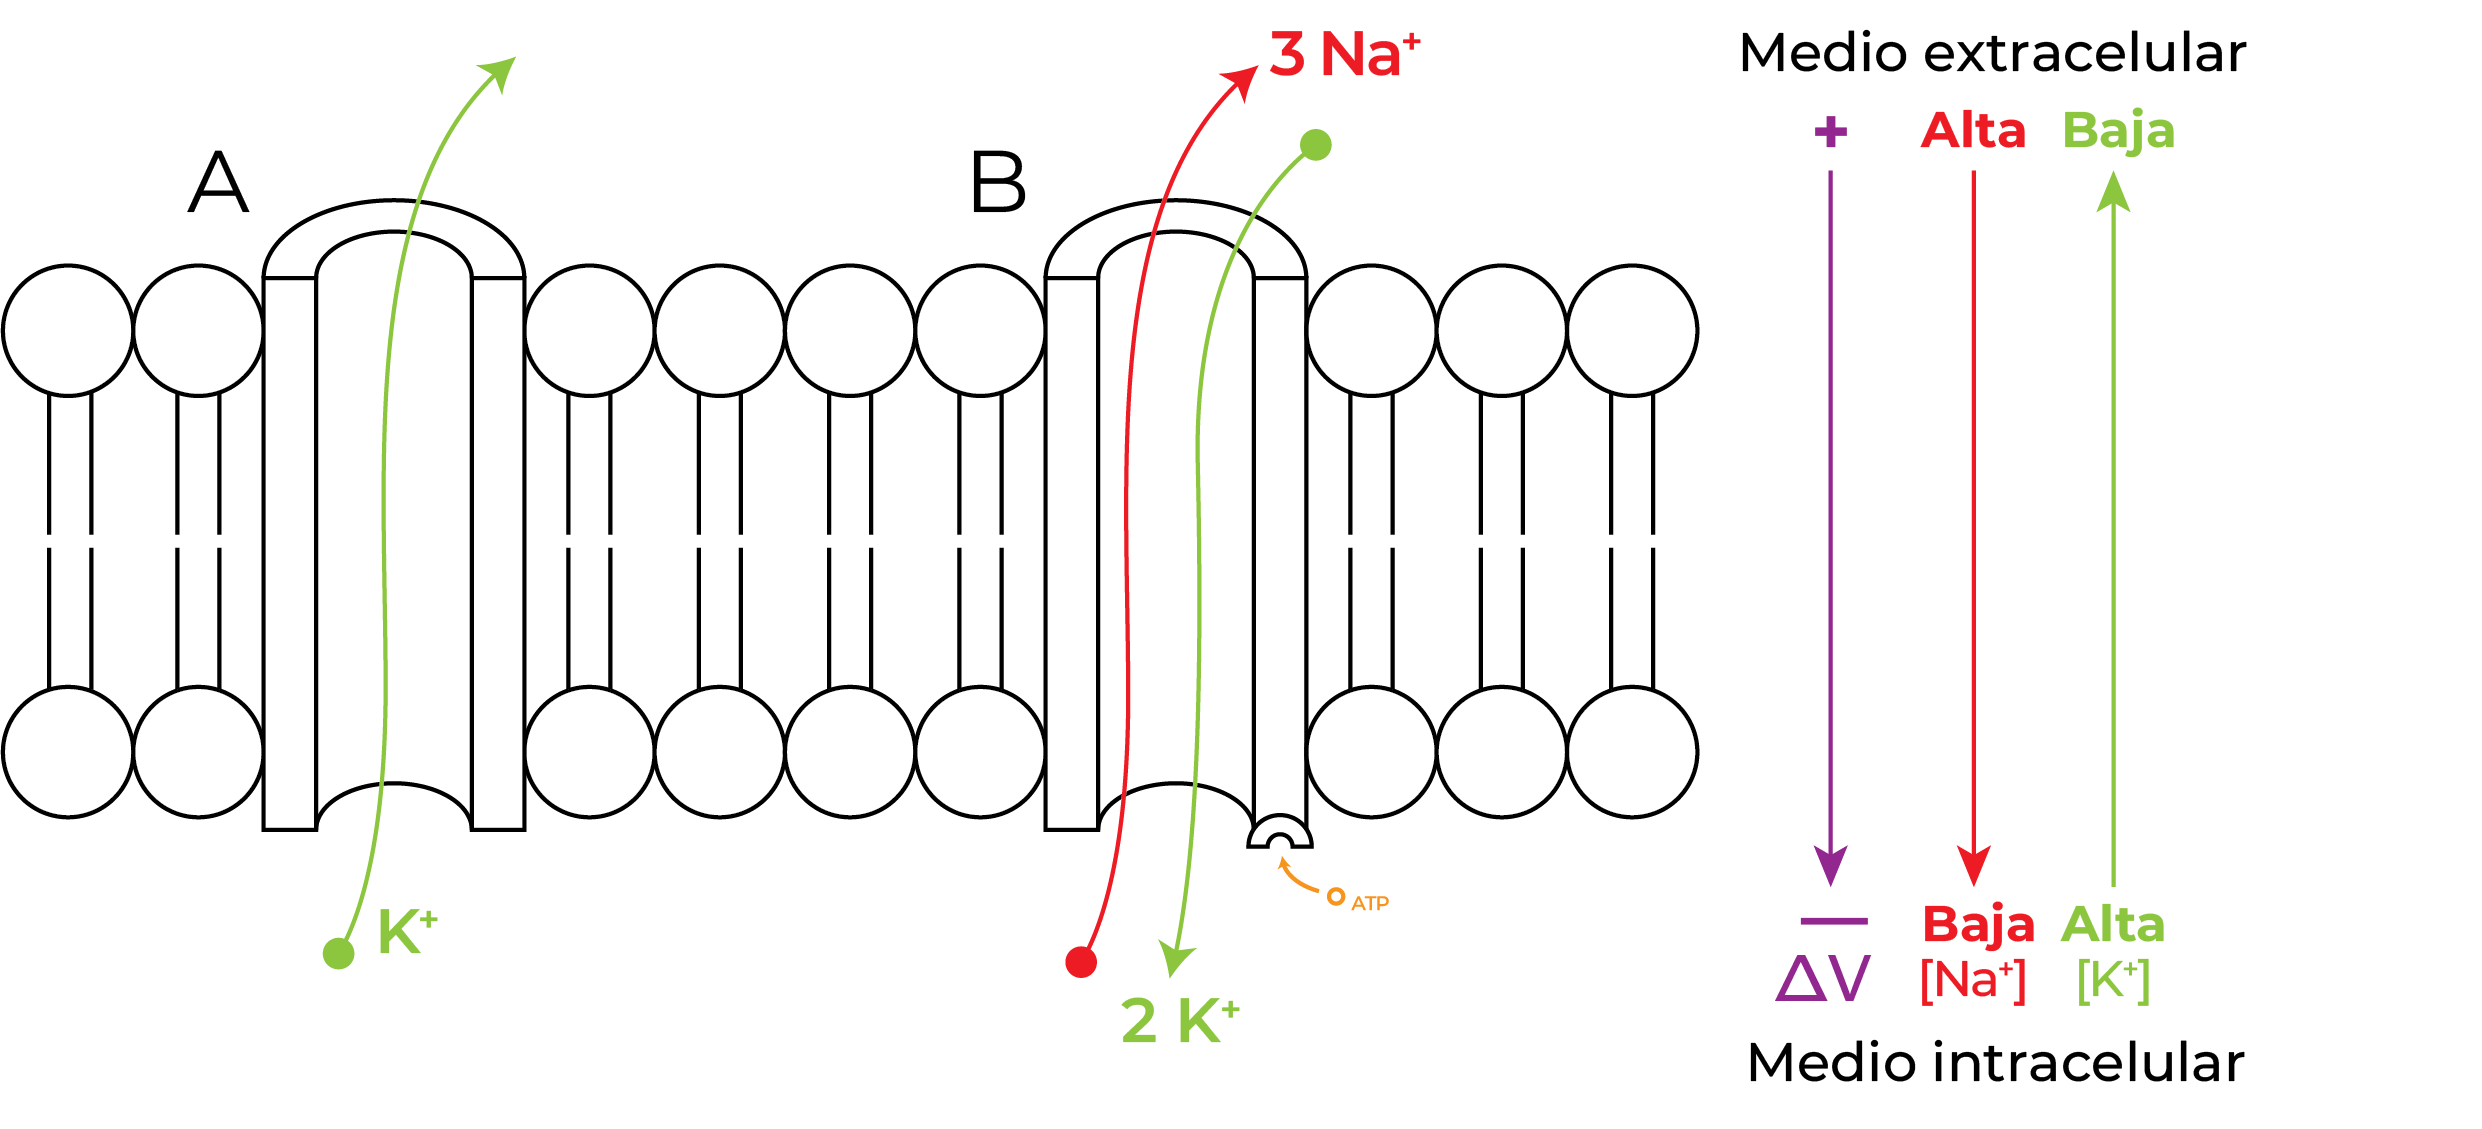
\includegraphics[width=\linewidth]{media/6-potencial.png}
	\caption{Transverse view of the neuron's membrane. IT contains potassium and sodium channels (A), which open mainly during the action potential. The Na$^+$-K$^+$ pump (B) maintains the inner concentrations of these ions.}
	\label{action}
\end{figure}

\begin{figure}[H]
	\centering
	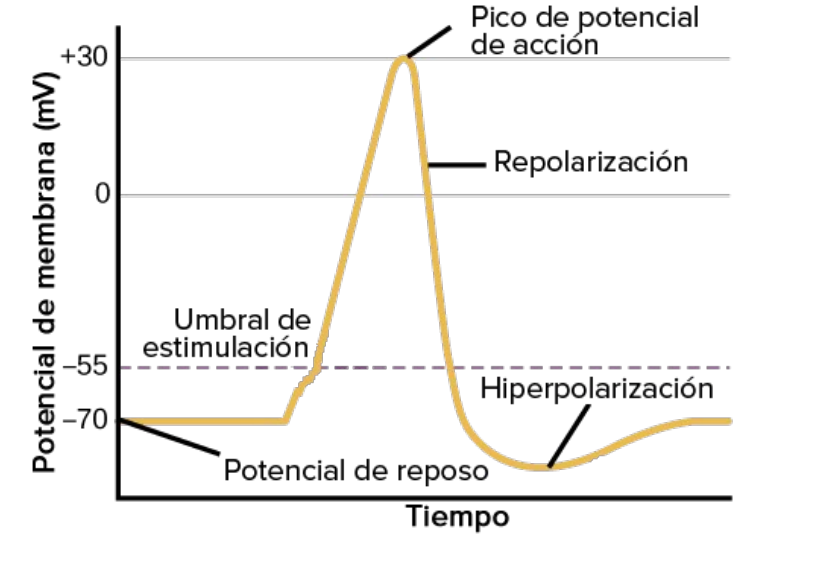
\includegraphics[width=\linewidth]{media/6-potencialgraph.png}
	\caption{Membrane potential through time.}
	\label{actiongraph}
\end{figure}

\subsection{Neurotransmission.}

Ion channels can open and close due to the joining of certain molecules we call \textit{neurotransmitters}. Each receptor corresponds to a single neurotransmitter. Neurotransmitters are released by the presynaptic neuron, which stores them in small vesicles. During the action potential, Ca$^{2+}$ channels open. The presence of calcium causes reactions over the vesicles' proteins and the cell membrane which produces the fusion of both (exocytosis). This fusion, which can be full or partial, frees up neurotransmitters contained in the vesicle into the synaptic space, where they travel until reaching receptors in the postsynaptic neuron, to which they join. Molecules that join to receptors are called \textit{ligands} (Figure \ref{synapse}).

When joining to receptors they can make it easier or harder for the channels to open, whether that be directly (on ionotropic receptors) or indirectly by producing metabolic changes in the cell (in metabotropic receptors). While it's true that the performed action depends on the receptor and less so on the transmitter, many neurotransmitters tend to be exclusively excitatory (they increase the chance for the channel to open, thereby increasing the chance that a signal is produced) or exclusively inhibitory (they decrease the chance). For example, aminoacids glutamate and GABA are the main components in charge of excitatory and inhibitory transmission respectively.

The most important neurotransmitters for our case are catecholamines (dopamine, norepinephrine and epinephrine), in charge of excitatory functions, fear, rage and reward; and serotonin: crucial in the regulation of mood, perception and dreams and very related to LSD.

\subsection{Example: the patellar reflex.}

The neural circuit that causes the knee-jerk reflex is a perfect example of what we've exposed so-far. With the leg flexed, the knee's tendon is striked. Its extension causes stress on the quadriceps, which causes an activation of sensory neurons, producing an excitatory afferent nervous impulse to the spinal cord. In the spinal cord, two efferent neurons are activated: an excitatory neuron to the quadriceps which releases acetylcholine on the muscle, a neurotransmitter responsible for its contraction; and an inhibitory neuron which avoids the activation of the analogous neuron in the complementary muscle: the hamstring (Figure \ref{sn}). This way, the quadriceps' contraction is coordinated with the hamstring's non-contraction (and hence extension), resulting in the leg extending. Excitatory neurons communicate using glutamate as neurotransmitter, inhibitory ones: GABA or glycine. The contraction of the muscle is mediated by the liberation of acetylcholine upon it.

\begin{figure}[H]
	\centering
	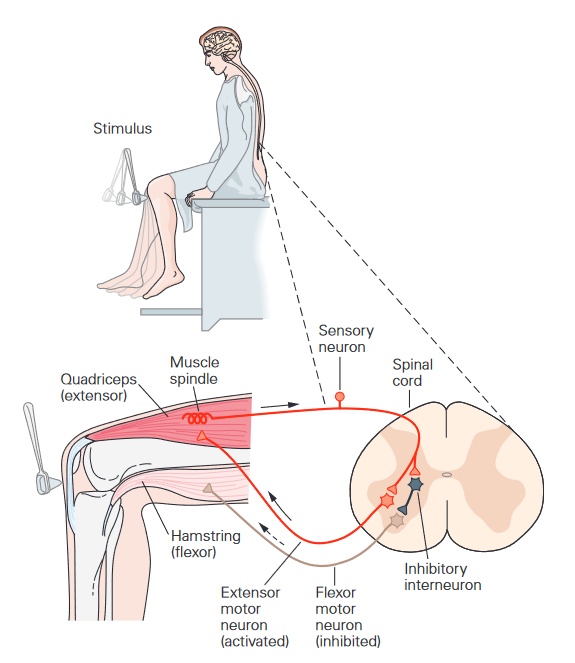
\includegraphics[width=.8\linewidth]{media/7-sn.png}
	\caption{The patellar reflex.}
	\label{sn}
\end{figure}

Like bees in a hive, the neurons get grouped in organizational levels more and more complex, producing faculties like senses and memory, building up the emergent phenomena that are the individual and --- maybe --- conscience.

In these more complex tasks we don't tend to bother with individual nerves and neurons, but rather observe how populations of neurons are activated in approximate regions on the encephalon. These regions can interact with each other. Sometimes they are associated anatomically, others functionally, and others by the neurotransmitter they use to communicate. That way, when someone is happy, there may be more activity in this or that region, whereas when they're scared, maybe the regions that secrete this or that neurotransmitter are inhibited.

Unfortunately, a \enquote{leap of faith} needs to be taken to establish a connection between psychology and neurobiology. This makes it very difficult to treat disorders related to the mind. Because the biological fundamentals behind them aren't fully understood, it isn't possbile to administer an infallible drug to cure them. This knowledge gap allows for the intrusion of shamanism and vedisms, although usually detached from their ritualistic-spiritual component in modern medicine.

\newpage
